
%%%%%%%%%%%%%%%%%%%%%%% file typeinst.tex %%%%%%%%%%%%%%%%%%%%%%%%%
%
% This is the LaTeX source for the instructions to authors using
% the LaTeX document class 'llncs.cls' for contributions to
% the Lecture Notes in Computer Sciences series.
% http://www.springer.com/lncs       Springer Heidelberg 2006/05/04
%
% It may be used as a template for your own input - copy it
% to a new file with a new name and use it as the basis
% for your article.
%
% NB: the document class 'llncs' has its own and detailed documentation, see
% ftp://ftp.springer.de/data/pubftp/pub/tex/latex/llncs/latex2e/llncsdoc.pdf
%
%%%%%%%%%%%%%%%%%%%%%%%%%%%%%%%%%%%%%%%%%%%%%%%%%%%%%%%%%%%%%%%%%%%


\documentclass[runningheads,a4paper]{llncs}

\usepackage{amssymb}
\usepackage{amsmath}
\setcounter{tocdepth}{3}

\usepackage{graphicx}
\graphicspath{{./pdf/}}
\DeclareGraphicsExtensions{.pdf}

\usepackage[caption=false,font=footnotesize,labelfont=sf,textfont=sf]{subfig}
\usepackage[ruled,vlined,linesnumbered]{algorithm2e}

\usepackage{url}
\usepackage{multirow,booktabs,makecell,color,colortbl}
 
\newcommand{\keywords}[1]{\par\addvspace\baselineskip
\noindent\keywordname\enspace\ignorespaces#1}

\begin{document}

\mainmatter  % start of an individual contribution

% first the title is needed
\title{A Heuristically Optimized Partitioning Strategy on Elias-Fano Index}

% a short form should be given in case it is too long for the running head
\titlerunning{A Heuristically Optimized Partitioning Strategy on Elias-Fano Index}

% the name(s) of the author(s) follow(s) next
%
% NB: Chinese authors should write their first names(s) in front of
% their surnames. This ensures that the names appear correctly in
% the running heads and the author index.
%
\author{Xingshen Song\inst{1} \and Kun Jiang\inst{2}\and  Yuexiang Yang\inst{1}}
%
\authorrunning{Xingshen Song, Kun Jiang, Jie He and Yuexiang Yang}
% (feature abused for this document to repeat the title also on left hand pages)

% the affiliations are given next; don't give your e-mail address
% unless you accept that it will be published
\institute{College of Computer, National University of Defense Technology,\\ Changsha, China\\
\email{\{songxingshen, yyx\}@nudt.edu.cn}
\and
School of Electronic and Information Engineering,\\ Xian Jiaotong University, Xian, China\\
\email{jk\_365@126.com}
}

% 
% NB: a more complex sample for affiliations and the mapping to the
% corresponding authors can be found in the file "llncs.dem"
% (search for the string "\mainmatter" where a contribution starts).
% "llncs.dem" accompanies the document class "llncs.cls".
%

\toctitle{A Heuristically Optimized Partitioning Strategy on Elias-Fano Index}
\tocauthor{Xingshen Song, Kun Jiang, Jie He and Yuexiang Yang}
\maketitle


\begin{abstract}
Inverted index is the preferred data structure for various query processing in large information systems, its compression techniques have long been studied to mitigate the dichotomy between space occupancy and decompression time.
During compression, partitioning posting list into blocks aligning to its clustered distribution, can effectively minimize the compressed size while keeping partitions separately accessed.
Traditional partitioning strategies using fixed-sized blocks trend to be easy to implement, but their compression effectiveness is vulnerable to outliers.
Recently researchers begin to apply dynamic programming to determine optimal partitions with variable-sized blocks.
However, these partitioning strategies sacrifice too much compression time.
%have overlooked using compression time as one criterion to evaluate their performances.
%Uniform partitioning with fixed-sized blocks is quite simple and crude, but it is tend to be vulnerable to outliers;
%Optimal partitioning with variable-sized blocks seems to remedy this defect but it is always too time consuming.

In this paper, we first compare performances of existing encoders in the space-time trade-off curve, then we present a faster algorithm to heuristically compute optimal partitions for the state-of-the-art Partitioned Elias-Fano index, taking account of compression time while maintaining the same approximation guarantees.
Experimental results on TREC GOV2 document collection show that our method makes a significant improvement against its original version.
%follow the state-of-the-art Partitioned Elias-Fano index by adopting the same approximation algorithm to prune back inefficient partitions, 
%made great progress by pruning inefficient partitions, we present a faster algorithm to heuristically compute optimal partitions, taking account of compression time while keeping the same approximation guarantees.
\keywords{Inverted Index, Index Compression, Partitioning Strategy, Approximation Algorithm}
\end{abstract}


\section{Introduction}
%Due to its simplicity and flexibility, inverted index gains a large amount of popularity among modern IR systems, especially in large scale search engines, inverted index is now adopted as the core component to fast respond to enormous queries. In its most basic and popular form, an inverted index is a collection of sorted lists of integers\cite{manning2008introduction,witten1999managing,zobel2006inverted}. Growing size of collection and high query efficiency requirement have appealed a large amount of research to compress the space occupancy of the index and speed up the query processing.
The performance of Information Retrieval systems rely largely on the data structure they adopt.
A well-designed data structure can juggle the mission of effectively storing related information and efficiently answering different kinds of queries.
Due to its simplicity and flexibility, inverted index gains more popularity than other candidates among modern IR systems since 1950s\cite{buttcher2010information,witten1999managing}, especially in large scale search engines.
However, as the rapid growth of the web, inverted index is facing an formidable performance challenge by billions of increasing documents and highly-concurrent queries.
Index compression is an important technique to mitigate such problem for it can yield a twofold advantage.
The immediate effect is that reduced space occupancy allows more data to be stored in limited store unit, more importantly, compression makes it possible to build in-memory index thus reducing the time of data transfer from slow memories\cite{manning2008introduction,zobel2006inverted}.

%the obvious reduction in space occupancy allows more data to be stuffed within a single store unit. On the other hand, by fitting more data into faster memory levels, compression reduces the size of data to be transferred from the slower levels. This is a classic example of trading CPU cycles for decreased I/O latency and bandwidth. For example, given the amount of computing power on a modern multi-core CPUs, transferring a compressed payload from the disk and decompress its content into memory is still far cheaper than just transferring the uncompressed data. Not only data transfers from disk to memory benefit from compression, also data transfers from memory to CPU is also positively affected by compression as it is shown by IBM Memory Expansion Technology [1]. This is a very well know fact also in IR where many scientific results show hot to exploit this trade-off [19, 18, 20, 13].

%inverted index is now adopted as their core component to maintain billions of documents and respond to enormous queries.
%In its most basic and popular form, an inverted index is a collection of sorted sequences of integers\cite{manning2008introduction,witten1999managing,zobel2006inverted}.
%Growing size of data and stringent query processing efficiency requirement have appealed a large amount of research, with the aim to compress the space occupancy of the index and speed up the query processing.

The inverted index can be seen as a collection of posting lists where each list $I_t$ is mapped to one term \textit{t} of vocabulary.
Inside $I_t$ are postings containing information about the occurrences of \textit{t} in one particular document \textit{d}, typically the \textit{docid}, the \textit{frequency}, and possibly the \textit{position} and other information.
These postings are always ordered by docid or frequency to fit different IR tasks\cite{navarro2010dual}.
To facilitate both compression and query processing, each list is treated as separate data stream and components inside are stored in a non-interleaved way\cite{anh2010index}. 

Many techniques for inverted index compression have been studied over years, see \cite{catena2014inverted,trotman2014compression} for more details.
Among these techniques, splitting posting list into blocks has been demonstrate to be an efficient way and widely adopted by many encoders.
For that by keeping blocks separately accessible we can expect faster decoding speed and hierarchical structure.
In addition, variable-sized blocks can utilize the clustering property of list to beat the entropy\cite{silvestri2010vsencoding,moffat2000binary}.
However, finding optimal partitions using variable-sized blocks can be very time consuming and the decoding procedure is delayed by additional cache miss.

%The compression techniques can be roughly divided into two categories,namely the \textit{integer-oriented encoders} and the \textit{list-oriented encoders}\cite{catena2014inverted,silvestri2010vsencoding}.
%The integer-oriented encoders assign an unique codeword to each integer of the posting list and are hard to decode because of plenty of bitwise operations.
%Recent work makes progress by optimizing byte/word-aligned encoders using SIMD instructions\cite{stepanov2011simd,trotman2014compression}.
%The list-oriented encoders are designed to exploit the cluster of neighboring integers and are much faster to decode, however, inferior in compression ratio.

While state-of-the-art techniques do obtain excellent space-time trade-offs, compression time is always neglected as one evaluating criterion. This can be attributed to the fact that index is always preprocessed offline before deployment, and once being taken into effect, update can be committed in an asynchronous and parallel manner. However, timely update for unexpected queries is becoming more and more stringent in search engine, traditional methods do not fit this scenario any more. Until recently researchers begin to use breakthroughs in compact data structure to bear on problems of optimizing inverted index\cite{navarro2010dual,ottaviano2014partitioned,petri2014score}.

\textit{Our contribution.}
We show that many encoders are far from optimal in terms of compression time while partitioned Elias-Fano index (PEF) yields a better trade-off than others, and we provide a heuristic partitioning strategy on PEF which computes partitions in a single pass with only one sliding window. We perform an experiment that shows index partitioned by our method is comparable to the original one.

%Compressing the index has long been a key issue for researchers to ensure both the time- and space-efficiency of inverted index, various encoders with different properties have been put up to settle this problem, and they can be roughly divided into two classes, namely the \textit{integer-oriented encoders} and the \textit{list-oriented encoders}. The integer-oriented encoders assign an unique codeword to each integer of the input sequence, then the compression procedure turns into a mapping or substitution from the integer space to code space. As they compress integers without considering their neighborings, the integer-oriented encoders are also called oblivious encoders\cite{catena2014inverted}, such as \textit{unary code, Elias Gamma/Delta codes \emph{and} Golomb/Rice codes}. Most integer-oriented encoders are hard to decode since they need bitwise operations to cross computer word boundaries, so byte/word-aligned encoders, are proposed to solve this problem, like \textit{Variable Byte} and \textit{Group Varint}, more importantly, they can be further improved by SIMD instructions of modern CPUs\cite{stepanov2011simd,trotman2014compression}.
%
%List-oriented encoders are designed to exploit the cluster of neighboring integers, each time a fixed-sized or variable-sized group of integers is binary packed with an uniform bit width, providing equivalent compression ratio and faster decoding speed, the technique used by these encoders is called \textit{frame-of-reference}(FOR), or \textit{binary packing}\cite{goldstein1998compressing}. Basically, their compression ratios are inferior to these of the first category as a batch of integers are encoded indiscriminately, and useless zeros are filled in the codeword to keep word-aligned, however, when decoded, list-oriented encoders can obtain an entire block while the formers just decode one integer at a time. More importantly, with the help of \textit{skip pointers} or \textit{skip list}, it is possible to step along the codewords compressed by list-oriented encoders and stop when the required number of blocks has been bypassed. Some of these encoders are \textit{Simple Family}, AFOR and \textit{Patched} FOR (PFOR, OptPFOR and FastPFOR).

%\section{Partitioning Strategies and Compression Criteria}
\section{Partitioning Strategies}
One thing to be noted is that list-oriented encoders may cost equivalent time to compress the posting list as the integer-oriented encoders even they are designed to compress a list of integers at the same time. Before compressing, a partitioning strategy needs to traverse the whole posting list to decide an optimal partition for compression ratio and decompression time, even after that, an uniform bit width is also needed to encode every element inside each block. Compression techniques like the Simple Family\cite{anh2005inverted,anh2010index}, enumerates all the possible partitioning cases to choose the suitable decision; OptPFOR\cite{yan2009inverted} needs an additional computation to choose the optimal proportion of exceptions in each block in order to achieve a better space efficiency. In the last few years there is a surge of partitioning schemes to accelerate the compression procedure\cite{lemire2015decoding,ottaviano2014partitioned}.

\textit{Directed Acyclic Graph.}
Blocks with fixed length are likely to be suboptimal as integers in posting list will not be evenly distributed.Works from literature\cite{anh2004index,delbru2012searching,silvestri2010vsencoding}give another perspective on partitioning. The posting list $\mathcal{S}[0,n-1]$ is considered a particular directed acyclic graph $\mathcal{G}$, each integer is represented by a vertex $v$, edge denoted as $\left( v_{i}, v_{j} \right)$ is an exact correspondence of a partition in the posting list $\mathcal{S}\left[i,j \right]$, edge has also associated its cost $c(v_{i},v_{j})=\left| \mathcal{E}\left(\mathcal{S}\left[i,j-1 \right] \right) \right| $ that corresponds to the size in bits of the partition compressed by encoder $\mathcal{E}$. Thus, the problem of optimally partitioning a list is reduced to the problem of Single-Source Shortest Path(SSSP) Problem.

However, a trivial traversal may not suffice to obtain an efficient solution for this problem, as the graph $\mathcal{G}$ is complete with $\Theta\left( n^{2}\right)$ edges, even partitioning posting lists with thousands of integers wi`ll be intolerable. Anh et al.\cite{anh2004index} and Delbru et al.\cite{delbru2012searching} adopt a greedy mechanism to partition the lists, the difference between them is that the former partitions the lists under a static table driven approach while the latter uses a set of fixed-sized sliding windows to determine. Fabrizio\cite{silvestri2010vsencoding} finds the optimal partition under a \textit{dynamic programming} approach but with limited options for partition lengths (say \textit{h}), reducing its time complexity from $O(n^{2})$ to $O(nh)$, but still barely satisfying in practice.

Since dynamic programming is inefficient and greedy mechanism is too coarse, a more feasible way will be using an elaborate approximation algorithm to find slightly suboptimal solutions, which reduce the time and space complexities to linear.
%an elaborate approximation algorithm will be feasible, which reduces the time and space complexities to linear, at the cost of finding slightly suboptimal solutions.

\section{Method Evaluation Criteria}
Compression techniques are optimized under two criteria, namely \textit{decompression time} and \textit{space occupancy}, different encoders yield different space-time trade-offs, generally, integer-oriented encoders tend to be more space-efficient while list-oriented encoders focus on time efficiency. \textit{Compression time} stays a low profile in the literature, as it does not make a difference for practical use, many encoders pursue a better performance at the expense of prolonging compression time, recently it begins to gain attention as one criterion to evaluate a compression technique\cite{lemire2015decoding,ottaviano2015optimal}.

\textit{Pareto-Optimal Compression.}
Taking the compression time into account, we get an extended tri-criteria to evaluate the performance of compression techniques. In this respect, we recall the concept of \textit{Pareto-optimal} compression to define the notion of ``best" compression in a principled way, i.e., encoders achieve different points in the space-time trade-off curve, optimal ones are those extreme points where performances are not worse than others in one dimension, and if to be optimized in any dimension, performances in the other two will get impaired accordingly. Absolutely there exists a set of Pareto-Optimal Compressions with different considerations. Figure~\ref{fig:performance} shows performances of different encoders\footnote{The installation of these implementations is same with the Experiments Section, even quite different from results in other work, but they are directly comparable with each other.}.

\begin{figure}
	\centering
	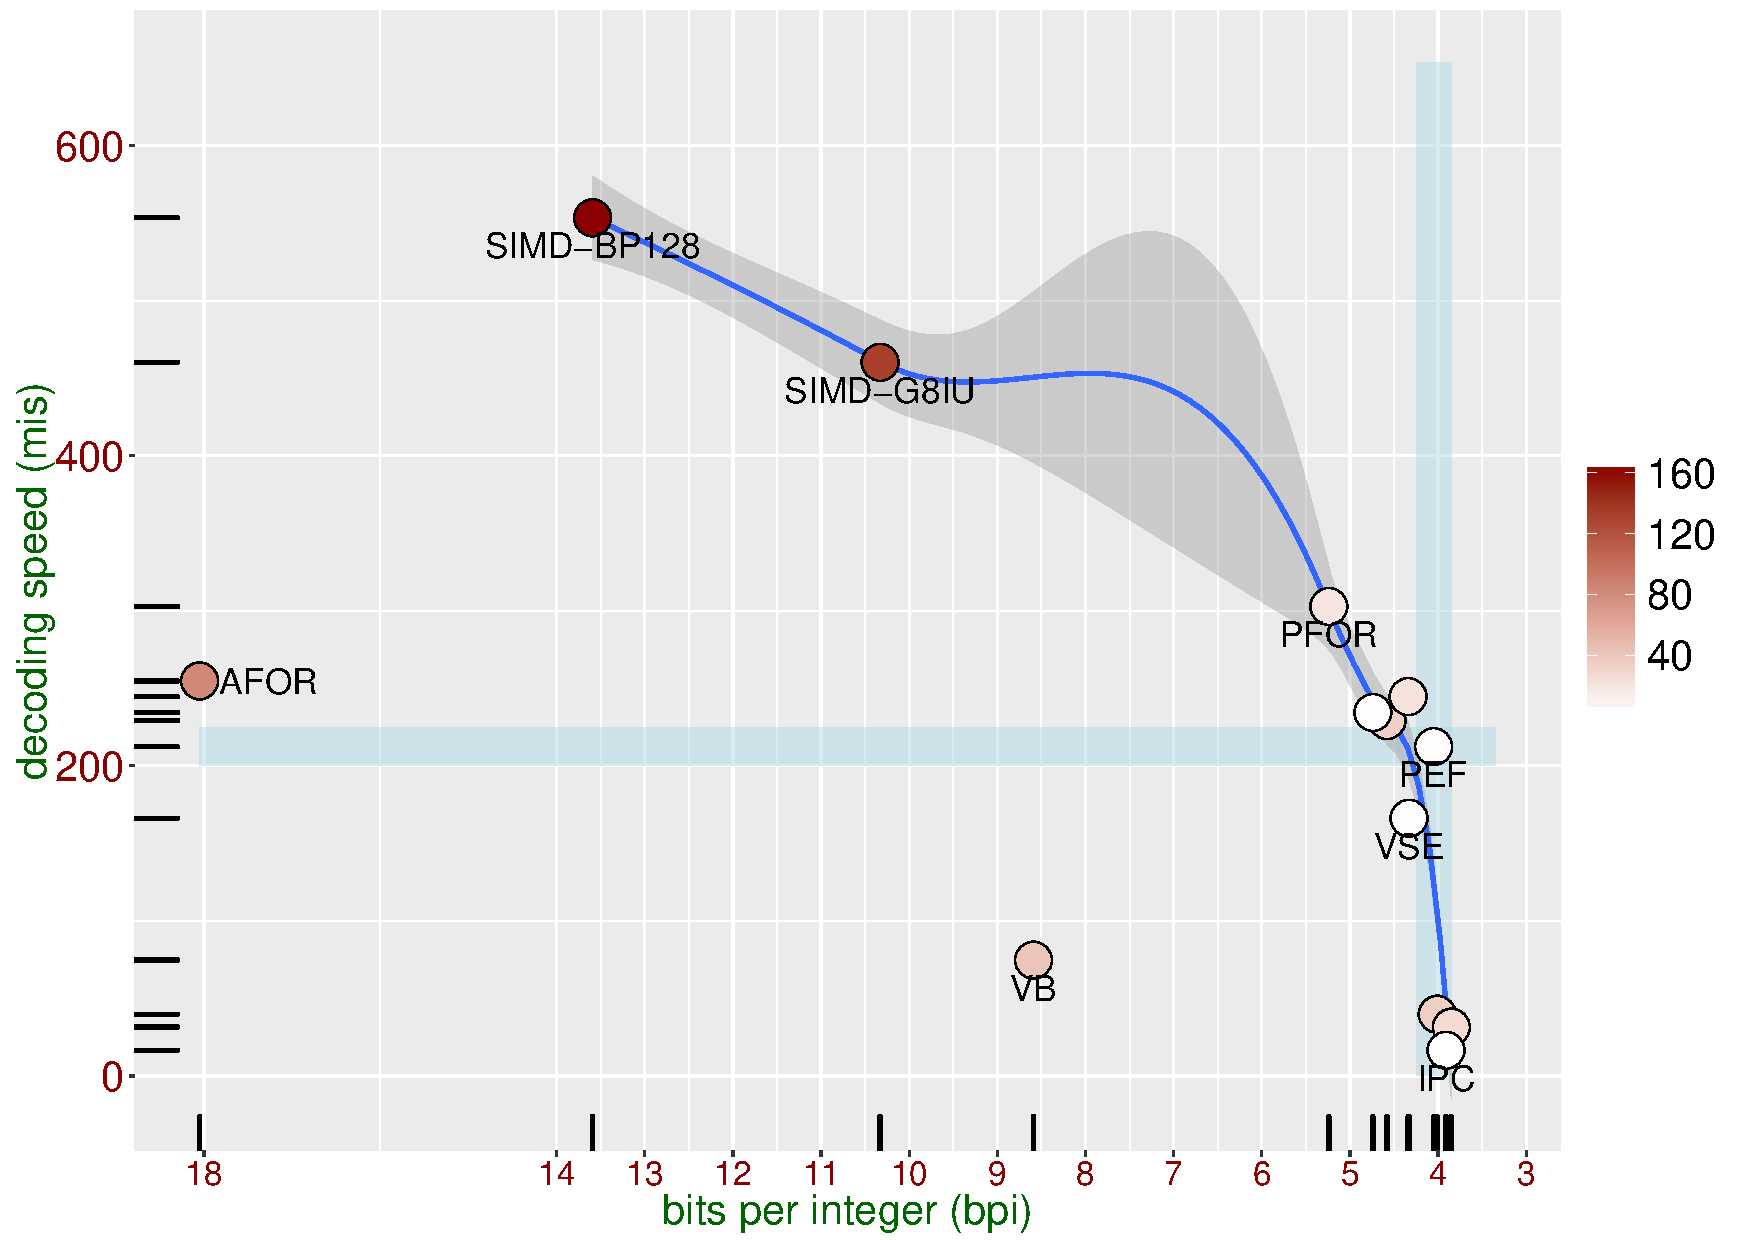
\includegraphics[width=0.7\linewidth]{performance}
	\caption{Performance of different encoders under tri-criteria. The x-axis (bpi) is arranged in a reverse order and color of each point indicates the encoding speed, the deeper, the faster.}
	\label{fig:performance}
\end{figure}

From the fitting curve and the marginal rugs, we can observe that points, which approach to limit of one dimension, begins to cluster and performances of the other two dimension drops intensely. Points beyond the curve are either superior or inferior to the average (i.e., VB and AFOR).

\textit{Partitioned Elias-Fano Index.}
We also emphasize PEF by two straight lines in Figure~\ref{fig:performance}, as it reaches a space occupancy competitive with integer-oriented encoders while keeping a reasonable decoding speed. It is a two-level data structure which partitions the posting list into Elias-Fano (EF) represented \textit{chunks} to adapt to its local statistics and stores pointers to these chunks in the upper EF sequence. Study shows that it is efficient in random access and search operations but slow in sequential decoding\cite{ottaviano2015optimal,vigna2013quasi}.

PEF describes a suboptimal partitioning strategy which finds the solution by generating a pruned DAG on the posting list in $O\left(n\log_{1+\varepsilon}\frac{1}{\varepsilon}\right)$ time and $O\left(\log_{1+\varepsilon}\frac{1}{\varepsilon}\right)$ space, and it is an $\left(1+\varepsilon\right)$-approximation algorithm to the optimal one, for any given $\varepsilon\in\left(0,1\right)$. However, it is still prohibitive in compression time, next section we describe a faster algorithm preserving the same approximation guarantee.

\section{Linear Partitioning Strategy}
% 这个地方复述的有点多,需要精简突出自己的method
\subsection{Partitioned Elias-Fano Index}
Given a monotonically increasing sequence $ \mathcal{S}[0,n-1] $ of $ n $ integers drawn from the range $ [0,u] $, and $ u $ is called an \textit{universe} of $ \mathcal{S} $. The Elias-Fano representation is a efficient quasi-succinct representation for monotone sequences used in \cite{elias1974efficient,vigna2013quasi}.
$ \mathcal{S} $ is represented using two bit arrays, namely \textit{the higher bits} and \textit{the lower bits}.
For a given integer $ \ell $, each element of $ \mathcal{S} $ is split into the lower $ \ell $ bits and the higher $ \lceil \log u \rceil - \ell$ bits.
The lower bits are stored explicitly and contiguously in the lower bits array \textit{L}, the higher bits are stored in the higher bits array \textit{H} as a sequence of unary-coded gaps (\cite{ottaviano2014partitioned} uses unary-coded buckets instead, but they both reach the same space complexity).
Thus, representing \textit{L} needs exactly $ n\ell $ bits, \textit{H} needs $ n + \frac{\lceil u \rceil}{2^{\ell}} $ bits. It has been shown that setting $ \ell = \lfloor \log \frac{u}{n} \rfloor $ minimizes the overall space of $ \mathcal{S} $, namely, at most $ n \lceil \log \frac{u}{n} \rceil + 2 n $ bits. Elements in Elias-Fano represented sequence are directly accessible by performing unary read on \textit{H} and direct read on \textit{L}, then merging them together.

However, Elias-Fano fails to exploit the distribution of clusters in the sequence as it treats $ \mathcal{S} $ as a whole.
We can actually expect for a better space occupancy when the sequence is formed by clusters of integers which are very close to each other.
This observation motivates the introduction of a two-level Elias-Fano, namely PEF, in which $ \mathcal{S} $ is first partitioned into chunks with variable lengths, then pointers to the head of each chunk are grouped together using Elias-Fano representation.
Partitioning the sequence aligning to its clusters will definitely narrow down the average distance of consecutive elements inside, thus a smaller compressed size is possible.
An optimal partition must satisfy the following two requirements: on one hand, the chunks should be as large as possible to minimize the number of pointers in upper level; on the other hand, the chunks should be as small as possible so as to narrow down the average distance.
However, traditional dynamic programming methods like \cite{silvestri2010vsencoding} turn out to be very costly when finding the optimal solution.
A more feasible way is adopting an approximation algorithm to prune the complete graph $ \mathcal{G} $ under some criteria, retaining its shortest path while cutting out edges which are impossible to be space-efficient.

Recall the approximation algorithm adopted in PEF, whose core idea is to generate a pruned subgraph $\mathcal{G}_{\varepsilon}\left(\mathcal{S}\right)$ of the original $\mathcal{G}\left(\mathcal{S}\right)$, the pruning strategy works by sparsifying edges in $\mathcal{G}\left(\mathcal{S}\right)$ into a geometric sequence with common ratio equals $(1+\varepsilon_{2})$, where $ \varepsilon_{2}\in\left(0,1\right) $, that is, for each vertex $v_{i}$ keeping the edge that approximates at the best the value $F\left(1+\varepsilon_{2}\right)^{k}$ from below for each integer $k$ ($F$ is the fixed cost of one partition).
By setting an upper bound $U$ (say, $U=\frac{F}{\varepsilon_{1}}$ by a predefined $\varepsilon_{1}\in\left(0,1\right)$), the total edges, addressed as $\varepsilon-maximal$ edges, in $\mathcal{G}_{\varepsilon}\left(\mathcal{S}\right)$ are $O\left(n\log_{1+\varepsilon}\frac{1}{\varepsilon}\right)$. 

\subsection{Heuristically Finding Optimal Partition}
These $\varepsilon-maximal$ edges can be found by keeping $k = O\left(\log_{1+\varepsilon}\frac{1}{\varepsilon}\right)$ sliding windows over $\mathcal{S}$.
During the algorithm visits posting list, the sliding windows are actually potential partitions, which start at the same position $ v_{i} $ but have different lengths.
At first, all these windows are docked at vertex 0 with 0 length.
Each time as the algorithm visits a subsequent vertex, these windows expand their sizes by appending this vertex to the end, once cost of the vertexes within current window, say $ \omega_{i} $, exceeds its threshold $ F \left( 1 + \varepsilon \right) ^{i} $, $ \omega_{i} $ stops expanding its size and we get one $\varepsilon-maximal$ edge of class $ i $.
Windows $ \omega_{i+1}, \dots, \omega_{k}$ will keep repeating this procedure until all the $\varepsilon-maximal$ edges out going from the starting vertex are figured out.
Then algorithm repeats the above procedure to find $\varepsilon-maximal$ edges for next vertex until reaches the end.
Given the fact that cost calculation can be done in constant time, it is easy to prove that returning an optimal partition only needs almost $ 2n\log_{1+\varepsilon}\frac{1}{\varepsilon} $ calls to cost calculation, namely in $O\left(n\log_{1+\varepsilon}\frac{1}{\varepsilon}\right)$ time.

However, it is still inefficient in practice since there can be tens of them, actually we need only one window to accommodate as many as possible integers and stop expanding as soon as an \textit{exception} is encountered.
The following lemma states a crucial property of the path over $\mathcal{G}\left(\mathcal{S}\right)$ to base our partitioning strategy on:	given any triple of indexes $i$, $j$ and $k$ in $\mathcal{G}$ with $0\leqslant i<j<k\leqslant n$, we have $c(v_{i},v_{j})\leqslant c(v_{i},v_{k})$ and $c(v_{j},v_{k})\leqslant c(v_{i},v_{k})$.

% 一旦发现不成比例的短路径,就证明这段间隔内存在异常值,就可以不再寻找接下来的路径了
We denote edges that start from $v_{i}$ over $\mathcal{G}_{\varepsilon}\left(\mathcal{S}\right)$ as $(v_{i},v_{j_{0}})$, $(v_{i},v_{j_{1}})$, \ldots, $(v_{i},v_{j_{k}})$, and for any adjacent two edges the ratio between them is $(1+\varepsilon_{2})$.
We speculate the lengths between them should also follow some regulations, an exception can enlarge the average distance inside an edge in a sudden, to keep its weight proportional to its former one, current edge's incremental length has to be comparatively small.
However, edges without exceptions should have their edge lengths growing proportionally.
A chunk that contains exception can be found by sequentially traversing these edges and comparing the incremental lengths.
Intuitively, an exception always leads to a short interval, and once we find this kind of interval a chunk can be built inside it, thus omitting exhaustive traversing all edges from one vertex to figure it out.
We can further shift the head of sliding window to the end of current chunk to skip more calculations.
As shown in Figure~\ref{fig:exceptions}.

\begin{figure}
	\centering
	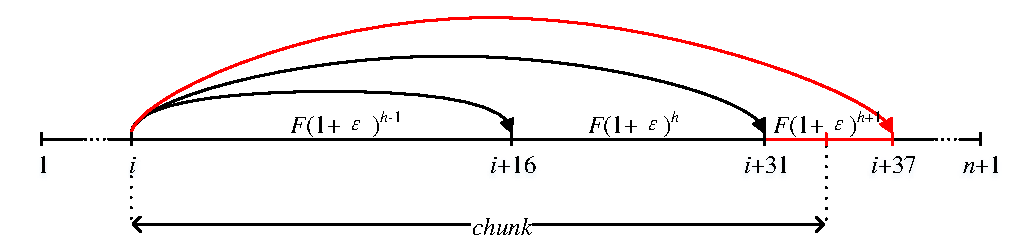
\includegraphics[width=1.0\linewidth]{exception}
	\caption{Finding $\varepsilon-maximal$ edges for position $ i $ using sliding windows. Here we show three edges with cost upper bound as $ F(1+\varepsilon)^{h-1}, F(1+\varepsilon)^{h}, F(1+\varepsilon)^{h+1} $, and their edge lengths are 16, 15, 6, respectively. Then we certain that an exception is encountered inside the third edge, and we can build a chunk right before the exception to save more space and reduce calculation.}
	\label{fig:exceptions}
\end{figure}

It remains to describe how to locate the chunk which contains exceptions, given a chunk $\left(v_{i},v_{j_{h}}\right)$, we only consider comparing with its former one, namely $\left(v_{i},v_{j_{h-1}}\right)$, inspired by Markov process.
Thus we have their partition lengths and partition universes as follow:
\begin{align}
n_{h} &= j_{h}-i, & u_{h} &= v_{j_{h}} - v_{i} \label{equ: chunk h}\\
n_{h-1} &= j_{h-1}-i, &  u_{h-1} &= v_{j_{h-1}} - v_{i}\label{equ: chunk h-1}
\end{align}
and their bit costs
\begin{equation}\label{equ: cost ratio}
{c\left(v_{i},v_{j_{h}}\right)}/{c\left(v_{i},v_{j_{h-1}}\right)}=1+\varepsilon_{2}
\end{equation}
However, different encodings are used in PEF to overcome the space inefficiencies of Elias-Fano in representing dense chunks.
A chunk $ \mathcal{P}_{h} $ is called a dense chunk if it covers a large fraction of the elements in the universe, that is $ n_{h} $ is close to $ u_{h} $.
As stated before, it will cost Elias-Fano $ n_{h} \lceil \log \frac{u_{h}}{n_{h}} \rceil + 2 n_{h} $ bits to represent $ \mathcal{P}_{h} $, nearly $ 2 u_{h} $ for a dense chunk.
In this case, a bitvector with a length $ u_{h} $ bits is a better choice, $ \mathcal{P}_{h} $ is represented by setting positions where integers happen to one.
And traditional \textit{rank/select} are also easy to implemented.
another extreme case is that chunk covers all the elements of universe $ u_{h} $, then we just need to store the partition length and partition universe while leaving the chunk non-encoded.
In spite of it is a fairly rare occurrence, once occurs it does sharply reduce the space occupancy.

To sum up, there are three representations $ \mathcal{E} $ for different chunks. $ \mathcal{E}=0 $: \textit{non-encoding} with $c\left(v_{i},v_{j_{h}}\right)=0$, if partition length $n_{h}$ equals to the universe $u_{h}$; $ \mathcal{E}=1 $: \textit{bitvector} with $c\left(v_{i},v_{j_{h}}\right)=u_{h}$, if $n_{h}\geqslant \frac{u_{h}}{4}$ and $ \mathcal{E}=2 $: EF with $c\left(v_{i},v_{j_{h}}\right)=n_{h}\lceil\log \frac{u_{h}}{n_{h}}\rceil+2n_{h}$, if $n_{h}<\frac{u_{h}}{4}$.
When we are about to identify chunks contain exceptions, we have to enumerate all the possible combinations of two consecutive chunks to find out corresponding reasonable incremental lengths.
That is, given Eq.~\eqref{equ: chunk h}~\eqref{equ: chunk h-1}~\eqref{equ: cost ratio}, we need to calculate $ \frac{n_h}{n_{h-1}} $ for $ \mathcal{E}[h-1] $ and $ \mathcal{E}[h] $, $ \mathcal{E} \in (0,1,2) $.
Actually there are only 4 combinations to consider since \textit{non-encoding} is unlikely to be leaded by the other two and more sensitive to exceptions.

Take $ \mathcal{E}[h-1]=1 $ and $ \mathcal{E}[h]=2 $ for example, then
\begin{displaymath}
\noindent
1+\varepsilon_{2}=\frac{n_{h}\lceil\log \frac{u_{h}}{n_{h}}\rceil+2n_{h}}{u_{h-1}}\geqslant \frac{n_{h}}{n_{h-1}}\cdot \frac{2+\log \frac{u_{h}}{n_{h}}}{4}>\frac{n_{h}}{n_{h-1}}.
\end{displaymath}
Others get the same conclusion by deduction
% (See the whole procedure in APPENDIX)
, so we set
\begin{equation}
\frac{u_{h}}{n_{h}}=1+\varepsilon_2
\end{equation}
as the same approximation factor with that of $\varepsilon-maximal$ edges.
Thus the whole procedure, which can be done within a single pass, is recast into using one window to expand its size from a starting vertex, building a chunk when current $\varepsilon-maximal$ edge is $\left(1+\varepsilon_{2}\right)$ times larger than the previous one and moving the starting vertex to $v_{h-1}+1$. A more space-efficient way is to traverse the interval $\left(v_{h},v_{h-1}\right)$ to determine a better cut-off vertex, which increases time complexity by no more than $\left(1+\varepsilon_{2}\right)$, and a minimum partition length is set to 8 to avoid slow-start and fragmentation of chunks.
Pseudo code of the above space-efficient procedure can be found in Algorithm~\ref{alg: optimal partition}.

\begin{algorithm} \label{alg: optimal partition}
	%	\SetAlgoNoLine
	\caption{Optimal partitioning}
	\KwIn{Posting list $ \mathcal{S}\left[1,n+1\right] $, fixed cost $ F $ and approximation factor $ \varepsilon_1, \varepsilon_2 $}
	\KwOut{Vector of optimal Partition $ P $}
	Initialize sliding window $ w $, $ bounds=\left\lbrace F,F(1+\varepsilon_2),F(1+\varepsilon_2)^2,\dots, \frac{F}{\varepsilon_1} \right\rbrace $, $ l=0 $, $ nS[bounds.size] $, $p\left[ n \right]$ and $min\_cost \left[n\right] $\;
	\For{$i=1;i<n+1;i$++}{
		$ min\_cost \left[i\right]=+\infty $\;
		$p[i]=0$\;
	}
	\While{$ w.end < n+1 $}{
		\While{true}{
			calculate cost of current window $ w.cost $\;
			\If{$ w.end == n+1 $}{
				$ p[w.end] = w.start $\;
				$ min\_cost \left[w.end\right]=min\_cost[w.start]+w.cost $\;
				\textbf{break}\;
			}
			\If{$ w.cost \geq bounds[l] $}{
				$ nS[l] = w.size $\;
				\If{$ l > 0\ \&\& \ nS[l-1] \geq 8 \ \&\& \ nS[l] < nS[l-1](1+\varepsilon_2) $}{
					create a chunk from $ w.start $ with a length $ nS[l-1] $, namely $ n_1 $\;
					move $ w.start $ forward $ nS[l-1] $\;
					\While{$ w.size > 1 $}{
						calculate $ w.cost $\;
						\If{$min\_cost \left[w.start\right]+ w.cost < min\_cost \left[w.end\right] $}{
							$min\_cost \left[w.end\right]=min\_cost[w.start]+w.cost $\;
							$ p[w.end]=w.start $\;
						}
						$ w.start++ $\;
					}
					$ l=0 $\;
					\textbf{break}\;
				}
				l++\;
				\If{$ l == bounds.size $}{
					create a chunk from $ w.start $ to $ w.end $\;
					move $ w.start $ to $ w.end $\;
					$ l=0 $\;
					\textbf{break}\;
				}
			}
			$ w.end++ $\;
		}
	}
	$ P=\left\lbrace p\left[n+1\right], p\left[p\left[n+1\right]\right], p\left[p\left[p\left[n+1\right]\right]\right],\cdots\right\rbrace $\;
	reverse the order of $ P $\;
	return $ P $\;
\end{algorithm}

\section{Experiments}
We use the posting lists extracted from the TREC GOV2 collection, which consists of 25.2 million documents and 32.8 million terms. All the terms have the Porter stemmer applied, stopwords are removed, and docids are reordered by the lexicographic order of URLs. All the implementations are carried out on an 8 core Intel(r) Xeon(r) E5620 processor running at 2.40 GHz with 128GB of RAM and 12,288KB of cache. Our algorithms are implemented using C++ and compiled with GCC 4.8.1 with -O3 optimizations. In all our runs, the whole inverted index is completely loaded into main memory, executions are reported as the mean of 4 consecutive replications.

We test performances of two strategies on EF index, \textit{coarse} which finishes partitioning in a single pass, and \textit{discreet} which works in a more space-efficient way, against the original methods, namely uniform-partitioned PEF (uniform) and $\varepsilon$-partitioned PEF (optimal).

First of all, We experiment differences caused by predefined parameters, namely the approximation $\varepsilon_{2}$ and the upper bound parameter $\varepsilon_{1}$. As coarse and discreet partition a posting list in a single pass, relying only on the total length. Construction time has little relevance to these parameters, and in practice it stays stable to them unsurprisingly. Figure~\ref{fig:parameter} shows the influences of them on index size, from which we can gain an insight into these two parameters: $\varepsilon_{2}$ determines the sensitivity to partitions which contains exceptions, and $\varepsilon_{1}$ determines the largest partition length which contains no exceptions, we can see index size is insensitive to $\varepsilon_{1}$ when it is nonzero, demonstrating the fact that most partitions cannot reach the largest length when encounter an exception. $\varepsilon_{2}$ used to be approximation bound, however index size is independent on it, as a small value will increase the number of partitions and a large one will yield too many long partitions. We set $\varepsilon_{2}=0.9$ and $\varepsilon_{1}=0.03$ in terms of performance.

\textit{Compression.} Table~\ref{tab: size and speed} shows the performances of different partitioning strategies, adding OptPFOR-compressed index (OptPFOR) as a baseline. It is clear that both proposed strategies outperform the original ones by a large margin over the compression time, making construction of PEF competitive with OptPFOR, at the cost of a slight larger space occupancy. Discreet has obvious superiority compared with coarse, sacrificing 4.7\% construction time in exchange for 6\% smaller index size, however, it still gets a better compression ratio than the last two uniformly partitioned indexes. The last column denotes time used for a sequential decompression of the index, discreet and coarse tends to use 10\% longer time to traverse the index than optimal and uniform, delayed by suboptimal partitions. Although all EF-based methods decompress much slower than OptPFOR, their advantages are embodied in random access when applied to query processing.

Table~\ref{tab: chunk size} shows comparisons of average partition lengths for different indexes, optimal has larger partition lengths but smaller index size than coarse and discreet, proving the fact it can better exploit the local clustering of the posting list. Discreet and coarse do not differ much from each other, as they can only approximately locate an exception and build a chunk in front of it. Next we show these lengths also influence query processing speed.

\begin{figure}
	\centering
	\subfloat[$\varepsilon_{2}=0$, varying $\varepsilon_{1}$ from 0 to 0.1]{
		\label{fig:phi:a}
		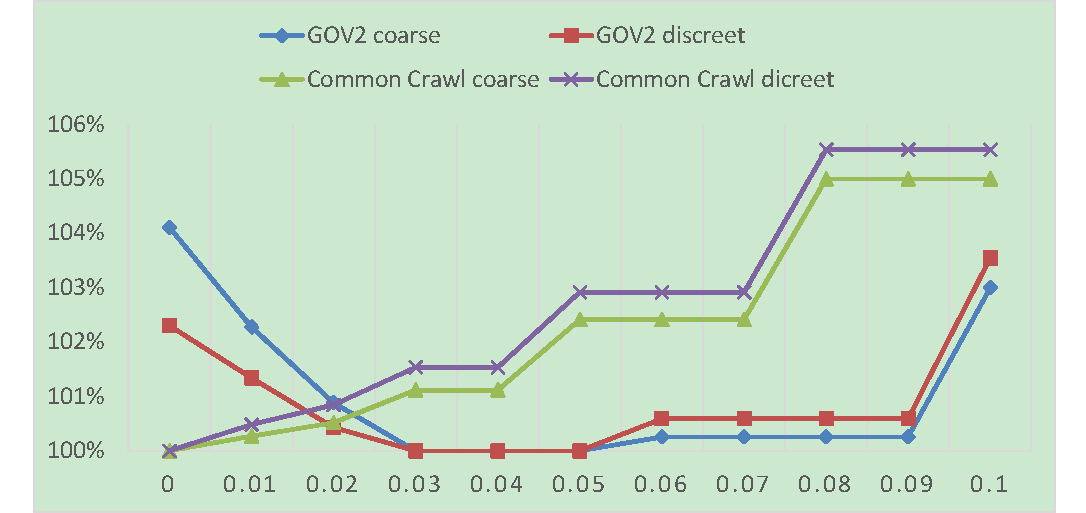
\includegraphics[width=0.7\linewidth]{eps1}
	}\\
	\subfloat[$\varepsilon_{1}=0.03$, varying $\varepsilon_{2}$ from 0.05 to 2]{
		\label{fig:epsilon:b}
		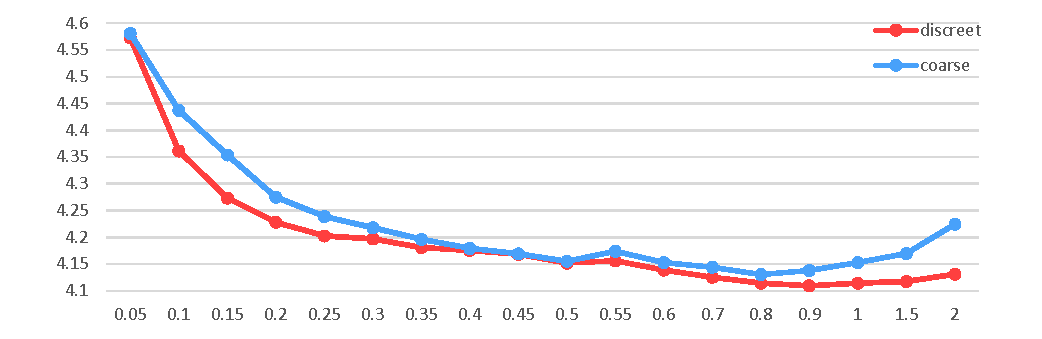
\includegraphics[width=0.7\linewidth]{eps2}
	}
	\caption{Influences of the parameters $\varepsilon_{2}$ and $\varepsilon_{1}$ on two partitioning strategies.}
	\label{fig:parameter}
\end{figure}

\begin{table}
	\centering
	\caption{Comparison of construction time, and average bits per element of each component}
	\renewcommand{\arraystretch}{1.0}
	\setlength\tabcolsep{9pt}
	\begin{tabular}{@{}l*{4}{r}} \toprule
		\multirow{2}*{methods} & \multicolumn{1}{c}{compress} & \multicolumn{1}{c}{docid} & \multicolumn{1}{c}{freq} & \multicolumn{1}{c}{decompress} \\
		&\multicolumn{1}{c}{\textbf{sec}} & \multicolumn{1}{c}{\textbf{bpi}} & \multicolumn{1}{c}{\textbf{bpi}} & \multicolumn{1}{c}{\textbf{sec}} \\ \midrule
		discreet & 870.70 & 4.40 & 2.32 & 99.46 \\
		coarse & 785.94 & 4.66 & 2.41 & 99.09 \\ \midrule
		optimal & 2638.91 & 4.05 & 2.19 & 86.11 \\
		uniform & 1615.94 & 4.63 & 2.40 & 88.61 \\
		OptPFOR & 688.90 & 4.55 & 2.34 & 49.43 \\
		\bottomrule
		\label{tab: size and speed}
	\end{tabular}
\end{table}

\begin{table}
	\centering
	\caption{Average partition lengths of different indexes for each component}
	\renewcommand{\arraystretch}{1.0}
	\begin{tabular}{@{}l*{5}{r}} \toprule
		& \multicolumn{1}{c}{optimal} & \multicolumn{1}{c}{coarse} & \multicolumn{1}{c}{discreet} & \multicolumn{1}{c}{uniform}& \multicolumn{1}{c}{OptPFOR} \\ \midrule
		docid & 208 & 194 & 187 & 128 & 128 \\
		freq  & 496 & 331 & 319 & 128 & 128 \\
		\bottomrule
		\label{tab: chunk size}
	\end{tabular}
\end{table}

\textit{Query efficiency.}
In order to explore the differences caused by partitioning strategies, the experiment adopts four widely-used methods of ranked query to find the top-20 results, DAAT\_AND, DAAT\_OR, WAND and Maxscore. We randomly select 4000 terms from the lexicon, any of which has a document frequency within the range $(10^{5},10^{6})$, and we regroup them into 1000 queries every 4 terms, avoiding the bias brought by short posting lists while highlighting advantage of random access.

As shown in Figure~\ref{fig:queries}, query time has been enlarged by involvements of multiple long posting lists, outliers can be as large as $10^{5}$ msec, however, most queries can be processed within hundreds of msec. Performances vary a lot among different processing methods,DAAT traverses the index in an exhaustive way, relying only on the throughput of postings. Needless to say, OptPFOR performs the best in DAAT and other indexes rank in accord with average partition lengths, the larger the length, the faster the speed. In detail, DAAT\_AND is the most efficient one as list intersection can cut off large of invalid postings, DAAT\_OR comes at a much higher cost as it cut nothing off, its rank also coincides with decompression speed shown in Table~\ref{tab: size and speed}. When it comes to dynamic pruning, PEF begins to gain an advantage over OptPFOR, also performance gaps among indexes again become unapparent, discreet and coarse even outperform optimal in WAND comparing both outliers and median. In general, results of different indexes do not differ much except those using DAAT\_OR, performances of discreet and coarse rank between optimal and uniform.

\begin{figure}
	\centering
	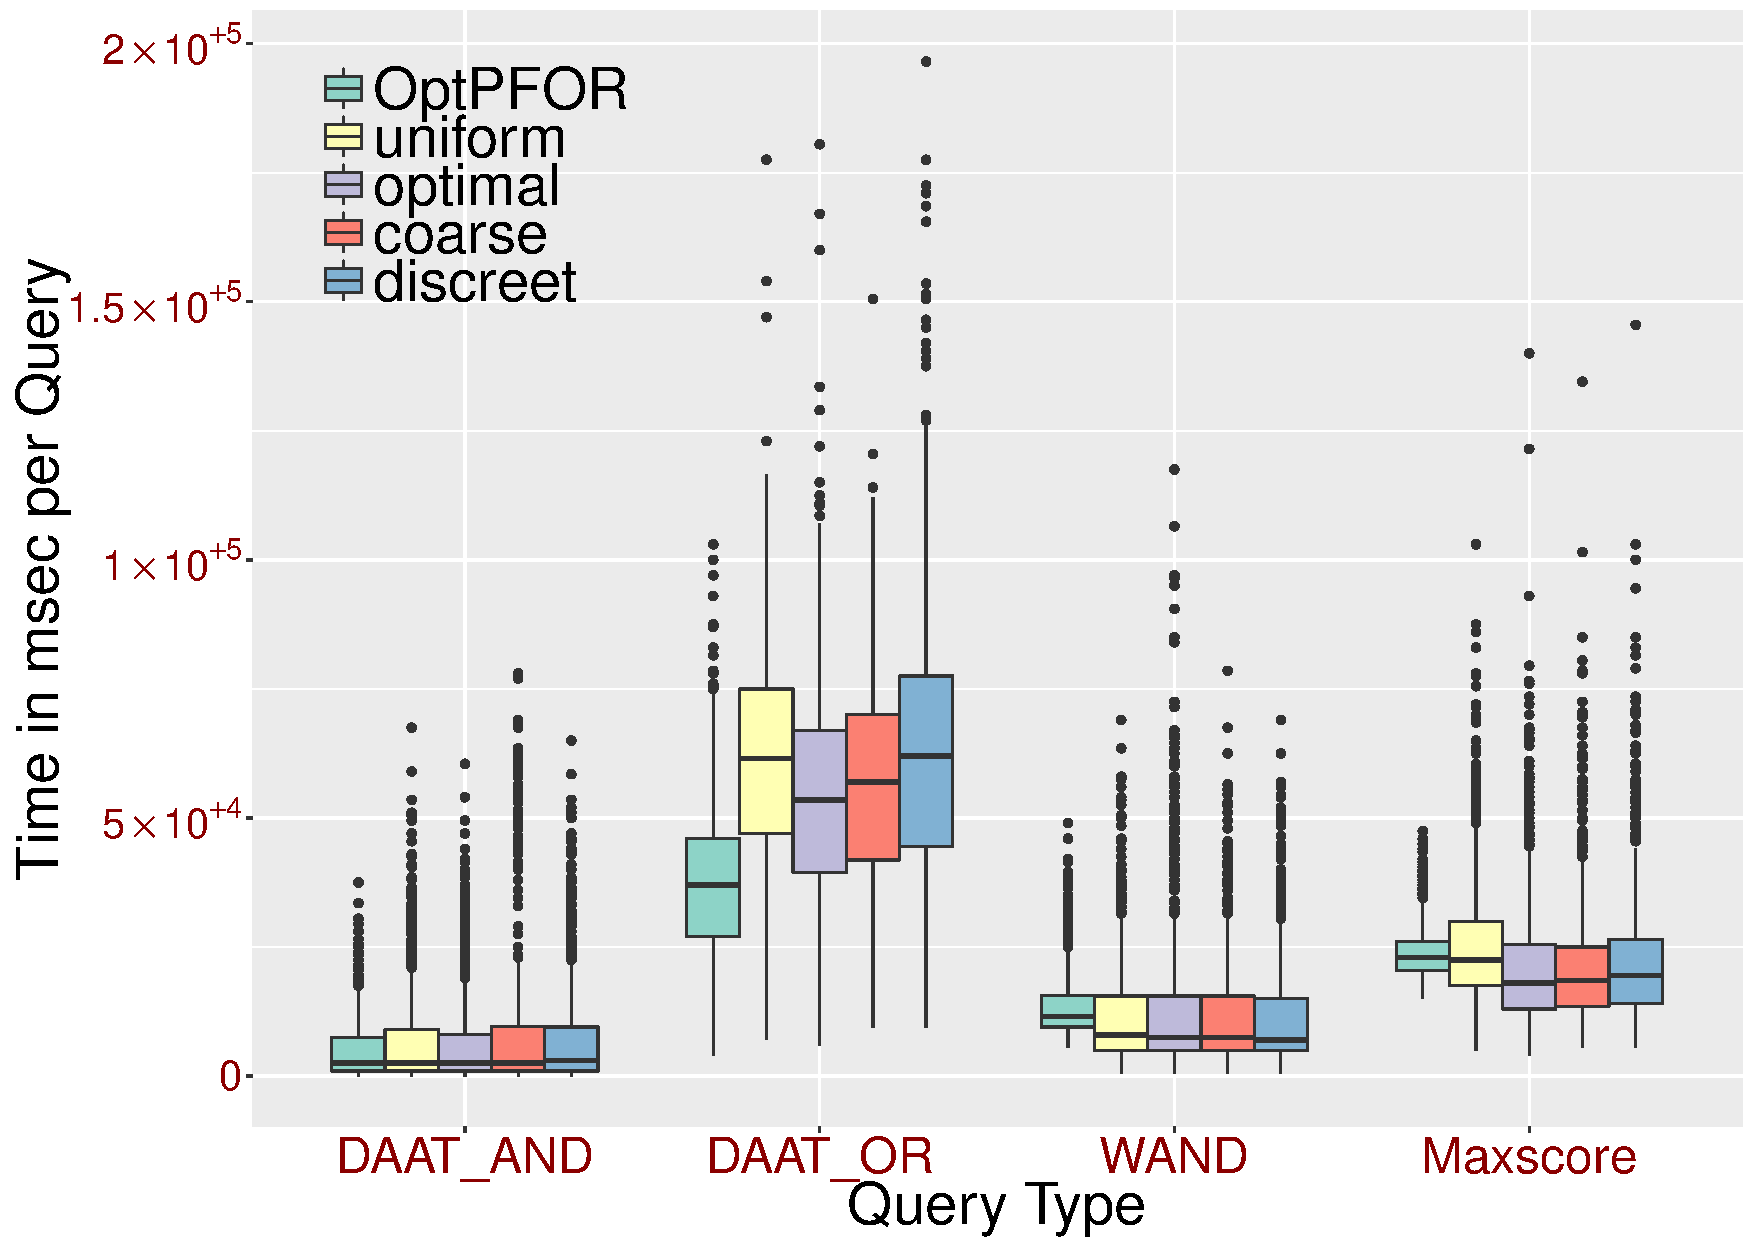
\includegraphics[width=0.7\linewidth]{queries}
	\caption{Query time distribution using different ranked query processing methods on candidate indexes.}
	\label{fig:queries}
\end{figure}

\section{Conclusion and Future Work}\label{sec:conclusion}

We have introduced the notion of Pareto-Optimal compression techniques taking compression time as one criterion and compared performances of different compressions. Our heuristic partitioning strategy over PEF gains lower time complexity while preserving same approximation guarantees,
%recently-proposed PEF gains a better space-time trade-off but slower construction speed, we then present a heuristic partitioning strategy with lower time complexity while preserving same approximation guarantees,
despite its simplicity, it does work well in practice when applied on GOV2.
%Experiments show its construction time is far more shorter than the originals while keeping competitive index size and query efficiency.
Future work will focus on formulating the notion of Pareto-Optimal Compression and exploring linear-time algorithms with different trade-offs under its criteria.

\bibliographystyle{splncs03}
\bibliography{reference}

\section*{Appendix: Deduction of reasonable partition length ratios}\label{apd}
%\appendix[Deduction of reasonable partition length ratios] 
Denote two consecutive partitions starting from the same position as $ \mathcal{P}_{1}[ v_0, v_1 ] $ and $ \mathcal{P}_{2}[v_0, v_2] $. Accordingly, their partition length and universe are $ n_1, u_1 $ and $ n_2, u_2 $, suppose $n_2 = n_1 + k, u_2 = u_1 + k + j $.
For completeness of exposition we report here the deduction of reasonable ratios for all the 9 combinations between $ \mathcal{E}[1] $ and $ \mathcal{E}[2] $, $ \mathcal{E} \in (0,1,2) $, showing that they asymptotically reaches the same upper bound as their partition cost. Shown as the following equation:

\begin{equation}
	\sup\{\frac{n_2}{n_{1}}\} = {c\left(v_{0},v_{2}\right)}/{c\left(v_{0},v_{1}\right)}=\frac{c_2}{c_1}=1+\varepsilon_{2}
\end{equation}

\begin{enumerate}
	
\item \label{itm: rb2rb}
Both chunks are represented using \textit{bitvector}, $ \mathcal{E}[1] = \mathcal{E}[2] = 1 $. Then
\begin{align*}
	c_2 & = u_2 & c_1 & = u_1 \\ 
	n_2 & > \frac{u_2}{4} &	n_1 & > \frac{u_1}{4}
\end{align*}
Since $ \frac{c_2}{c_1}=1+\varepsilon_2, n_2 = n_1 + k, u_2 = u_1 + k + j  $, we get
\begin{gather*}
	\frac{u_2}{u_1} = \frac{u_1+k+j}{u_1}=1+\varepsilon_2\\
	\frac{u_1+k+j}{n_1+k} < 4\\
	\frac{u_1}{n_1} < 4
\end{gather*}
Finally
\begin{gather*}
k+j<4k<4n_1\cdot \varepsilon_2 \\
\frac{n_2}{n_1}=\frac{n_1+k}{n_1} < \frac{n_1+ n_1\cdot \varepsilon_2}{n_1}=1+\varepsilon_2
\end{gather*}

\item \label{itm: ef2ef}
Both chunks are represented using EF, $ \mathcal{E}[1] = \mathcal{E}[2] = 2 $. Then
\begin{align*}
c_2 & = n_2(2+\lfloor \log \frac{u_2}{n_2} \rfloor) & c_1 & = n_1(2+\lfloor \log \frac{u_1}{n_1} \rfloor) \\ 
n_2 & \leq \frac{u_2}{4} &	n_1 & \leq \frac{u_1}{4}
\end{align*}
Since
\begin{gather*}
	\frac{n_2}{n_1} \cdot \frac{2+\lfloor \log \frac{u_2}{n_2} \rfloor}{2+\lfloor \log \frac{u_1}{n_1} \rfloor} = 1 + \varepsilon_2 \\ 
	\lfloor \log \frac{u_2}{n_2} \rfloor \geq 2 \Rightarrow \frac{2+\lfloor \log \frac{u_2}{n_2} \rfloor}{2+\lfloor \log \frac{u_1}{n_1} \rfloor} \approx 1
\end{gather*}
We get 
\[
 \frac{n_2}{n_1} \approx 1+ \varepsilon_2 
\]

\item \label{itm: rb2ef}
The former chunk is represented by \textit{bitvector} and the latter is EF,$ \mathcal{E}[1]= 1, \mathcal{E}[2]=2 $. Then
\begin{align*}
c_2 & = n_2(2+\lfloor \log \frac{u_2}{n_2} \rfloor) & c_1 & = u_1 \\ 
n_2 & \leq \frac{u_2}{4} &	n_1 & > \frac{u_1}{4}
\end{align*}
Since
\begin{gather*}
\frac{n_2 \cdot (2+\lfloor \log \frac{u_2}{n_2} \rfloor)}{4 n_1} < \frac{n_2 \cdot (2+\lfloor \log \frac{u_2}{n_2} \rfloor)}{u_1} = 1 + \varepsilon_2 \\
\frac{n_2}{n_1} \cdot \frac{2+\lfloor \log \frac{u_2}{n_2} \rfloor}{4} < 1 + \varepsilon_2
\end{gather*}
we get
\[
	\frac{n_2}{n_1} \leq \frac{n_2}{n_1} \cdot \frac{2+\lfloor \log \frac{u_2}{n_2} \rfloor}{4} < 1 + \varepsilon_2
\]

\item \label{itm: ef2rb}
The former chunk is represented by EF and the latter is \textit{bitvector},$ \mathcal{E}[1]= 2, \mathcal{E}[2]=1 $. Then
\begin{align*}
c_2 & = u_2 & c_1 & = n_1(2+\lfloor \log \frac{u_1}{n_1} \rfloor)\\ 
n_2 & > \frac{u_2}{4} & n_1 & \leq \frac{u_1}{4}
\end{align*}
Since
\begin{gather*}
\frac{4 n_2}{n_1 \cdot (2+\lfloor \log \frac{u_1}{n_2} \rfloor)} > \frac{n_2 \cdot (2+\lfloor \log \frac{u_2}{n_2} \rfloor)}{u_1} = 1 + \varepsilon_2 \\
\frac{n_2}{n_1} \cdot \frac{4}{2+\lfloor \log \frac{u_1}{n_1} \rfloor} > 1 + \varepsilon_2
\end{gather*}
we get
\[
\frac{n_2}{n_1} \geq \frac{n_2}{n_1} \cdot \frac{2+\lfloor \log \frac{u_2}{n_2} \rfloor}{4} > 1 + \varepsilon_2
\]
\end{enumerate}

Note that chunks represented using \textit{bitvector} are dense chunks, those using EF are sparser.
So in previous case~\ref{itm: rb2ef}, chunks change from dense to sparse, exceptions are certainly encountered in the middle.
As for case~\ref{itm: ef2rb}, chunks are becoming dense, it only happens under the situation with out exceptions.

We do not analyze chunks represented using \textit{non-encoding}, as they extreme cases that are rarely encountered, and their partition weights are set to be zero which makes them more sensitive to exceptions.
Intuitively, \textit{non-encoding} cannot be leaded by EF or \textit{bitvector}, and it can be followed by the other two representations no matter how long its partition length is.
In extreme case, we can set every single integer to be represented by \textit{non-encoding}, however, it does not compress at all and produces many more chunks. So chunks using \textit{non-encoding} are set to be at least longer than 8 integers and following the same upper bound as other cases.

Thus we set the partition length ratio to be $ 1+\varepsilon_2 $, and once $ \frac{n_2}{n_1} < 1+ \varepsilon_2 $ for two consecutive chunks starting from the same position, we can certainly determine that an exception is encountered in the middle.  

\end{document}
